%%%%%%%%%%%%%%%%%%%%%%%%%%%%%%%%%%%%%%%%%%%%%%%%%%%%%
%                                                   %
%     Penn State Colloquium Poster Template         %
%                                                   %
% Uses Penn State Colloquium class, with options:   %
%                                                   %
% Orientation:                                      %
%     portrait (default), landscape                 %
%                                                   %
% Paper size:                                       %
%     a4paper (default), a0paper, a1paper, a2paper, %
%     a3paper, a5paper, a6paper                     %
%%%%%%%%%%%%%%%%%%%%%%%%%%%%%%%%%%%%%%%%%%%%%%%%%%%%%
\documentclass{../psuposter}
\renewcommand{\templateimagepath}{../} 


%%%%%%%%%%%%%%%%%%%%%%%%%%%%%%%%%%%%%%%%%%%%%%%%%%%%%
%               Package Dependencies                %
%%%%%%%%%%%%%%%%%%%%%%%%%%%%%%%%%%%%%%%%%%%%%%%%%%%%%
\usepackage{natbib}
\usepackage{lipsum}                                % Dummy text
\usepackage[figwidth = 0.98\linewidth]{todonotes}  % Dummy image (and more!)
\usepackage[absolute, overlay]{textpos}            % Figure placement
\usepackage{braket}
\setlength{\TPHorizModule}{\paperwidth}
\setlength{\TPVertModule}{\paperheight}
\setcitestyle{numbers,square}


%%%%%%%%%%%%%%%%%%%%%%%%%%%%%%%%%%%%%%%%%%%%%%%%%%%%%
%                 AUTHOR AND TITLE                  %
%%%%%%%%%%%%%%%%%%%%%%%%%%%%%%%%%%%%%%%%%%%%%%%%%%%%%
\title{What Do Quantum Defects Talk About? (and how can we find out?)}
\author{Evelyn Hu}
\institute{Harvard University}


%%%%%%%%%%%%%%%%%%%%%%%%%%%%%%%%%%%%%%%%%%%%%%%%%%%%%
%                  BEGIN DOCUMENT                   %
%%%%%%%%%%%%%%%%%%%%%%%%%%%%%%%%%%%%%%%%%%%%%%%%%%%%%
\begin{document}
\begin{frame}
\begin{columns}[t, totalwidth=\textwidth]
\begin{column}{0.45\textwidth - 1cm}


%%%%%%%%%%%%%%%%%%%%%%%%%%%%%%%%%%%%%%%%%%%%%%%%%%%%%
%                 BLOCK: BIOGRAPHY                  %
%%%%%%%%%%%%%%%%%%%%%%%%%%%%%%%%%%%%%%%%%%%%%%%%%%%%%
    \begin{block}{Speaker Biographic Summary}
    	\begin{center}
    		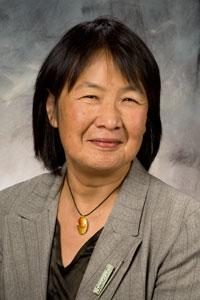
\includegraphics[width=0.5\textwidth]{images/portrait}
    	\end{center}
    	\href{https://hugroup.seas.harvard.edu}{Dr. Evelyn Hu} is the Tarr-Coyne Professor of Applied Physics and of Electrical Engineering at Harvard University. Hu received a B.A. in Physics from Barnard College, and completed her Ph.D. in Physics from Columbia University. Prior to her appointment at Harvard, she was Scientific Co-Director, California Nanosystems Institute and a Professor in the Departments of Electrical and Computer Engineering and Materials at the University of California, Santa Barbara. She also worked at AT\&T Bell Laboratories. Hu is a member of the National Academy of Sciences, National Academy of Engineering, American Academy of Arts and Sciences, the Academica Sinica of Taiwan, a recipient of an NSF Distinguished Teaching Fellow award, an AAAS Lifetime Mentor Award, a Fellow of the IEEE, APS, and the AAAS.
    \end{block}


%%%%%%%%%%%%%%%%%%%%%%%%%%%%%%%%%%%%%%%%%%%%%%%%%%%%%
%            BLOCK: RESEARCH INTERESTS              %
%%%%%%%%%%%%%%%%%%%%%%%%%%%%%%%%%%%%%%%%%%%%%%%%%%%%%
    \begin{block}{Research Interests}
        Dr. Hu's research matches nanofabrication techniques with the integration of materials that allow the formation of structures and devices that demonstrate exceptional electronic and photonic behavior. This behavior can give rise to efficient, controlled and often coherent output of devices. One example of this is the focus on coupling artificial atoms, such as quantum dots or color centers in diamond, to carefully-crafted nanoscale optical cavities. 
        \begin{center}
	    	
\includegraphics[width=0.65\textwidth]{images/research}    		

    	\textit{Real space images of a disk pair in uncoupled mode. \cite{seyfferleSignaturesSinglephotonInteraction2018}} 
    	\end{center}
    \end{block}
\end{column}
\begin{column}{0.55\textwidth - 1cm}


%%%%%%%%%%%%%%%%%%%%%%%%%%%%%%%%%%%%%%%%%%%%%%%%%%%%%
%                 BLOCK: ABSTRACT                   %
%%%%%%%%%%%%%%%%%%%%%%%%%%%%%%%%%%%%%%%%%%%%%%%%%%%%%
    \begin{block}{Talk Abstract}
    	There has been recent excitement about the performance of defects (such as vacancies, or missing atoms) in crystalline semiconductors, where the defect, also termed qubit, can manifest optical emission at a variety of wavelengths, distinctively coupled to long spin coherence times. The deliberate creation of such defects, for example with ion beam irradiation, almost certainly implies the creation of “collateral” defects and disorder to the surrounding environment: how does this affect luminescence efficiency, spin coherent lifetimes and other important qubit metrics?

		This talk will focus on Silicon Vacancies in 4H SiC, integrated into “bespoke” nanoscale optical cavities, with an effective volume of about (100 nm)3. The cavities serve to augment the optical signal by orders of magnitude, but also serve as “nanoscopes” into the material, allowing us to learn about the interactions with surrounding defects, and giving us broader insights into longer-term quantum coherence.
    \end{block}


%%%%%%%%%%%%%%%%%%%%%%%%%%%%%%%%%%%%%%%%%%%%%%%%%%%%%
%                BLOCK: BACKGROUND                  %
%%%%%%%%%%%%%%%%%%%%%%%%%%%%%%%%%%%%%%%%%%%%%%%%%%%%%
    \begin{block}{Brief Background}
    	Quantum interconnects (QuICs) are devices that allow the transfer of quantum states between two specified physical degrees of freedom (material, electromagnetic, etc.), or, more broadly, connect a quantum system with a classical one. \cite{awschalomDevelopmentQuantumInterconnects2021} 
%    	Figure 1 shows a schematic of a network of diverse quantum infor- mation systems, central to which is a quantum switch (QS)—a device that can route optical signals between dif- ferent channels while maintaining quantum coherence and entanglement  
    	%\cite{longLocalAxonalConduction2020} 
        \begin{center}
		   	
\includegraphics[width=0.8\textwidth]{images/background}    		

			\textit{The broad role of QuICs in quantum information technology. \cite{awschalomDevelopmentQuantumInterconnects2021}}
    	\end{center}
		An entangled quantum state of two or more objects describes their joint state and thus their statistically correlated measured properties, with correlations that are stronger than possible according to classical physics. Entanglement is the essential resource that enables nearly all quantum technology, but is very fragile, making it hard to create and maintain over long times and across large distances. \cite{awschalomDevelopmentQuantumInterconnects2021}
		%\cite{longMorphologicalCharacterizationHVC2018} 
    \end{block}


%%%%%%%%%%%%%%%%%%%%%%%%%%%%%%%%%%%%%%%%%%%%%%%%%%%%%
%                 BLOCK: REFERENCES                 %
%%%%%%%%%%%%%%%%%%%%%%%%%%%%%%%%%%%%%%%%%%%%%%%%%%%%%
    \begin{block}{References}
        \bibliographystyle{aipnum4-1}
%        \bibliographystyle{iopart-num}
		\bibliography{references}
    \end{block}

\end{column}
\end{columns}


%%%%%%%%%%%%%%%%%%%%%%%%%%%%%%%%%%%%%%%%%%%%%%%%%%%%%
%                    FOOTER TEXT                    %
%%%%%%%%%%%%%%%%%%%%%%%%%%%%%%%%%%%%%%%%%%%%%%%%%%%%%
\begin{textblock}{0.5}(0.18, 0.94)
    \color{white}
    \sffamily
    \textbf{Eberly College of Science}
    \\
    Department of Physics
\end{textblock}


%%%%%%%%%%%%%%%%%%%%%%%%%%%%%%%%%%%%%%%%%%%%%%%%%%%%%
%                   END TEMPLATE                    %
%%%%%%%%%%%%%%%%%%%%%%%%%%%%%%%%%%%%%%%%%%%%%%%%%%%%%
\end{frame}
\end{document}
